\documentclass{article}


\usepackage{amsmath,amssymb,graphicx,xcolor,xepersian}

\newcommand{\qn}[1]{
\[
\begin{split}
#1
\end{split}
\]
}

\begin{document}

%{
%\centering
%به نام زیبایی
%
%کوئیز 2 درس سیگنال ها و سیستم ها
%}

\large

الف)

تبدیل z سیگنالهای 
$
(\frac{2}{3})^nu[n]
$
و
$
(\frac{4}{3})^nu[-n-1]
$
به ترتیب برابر 
$
\frac{1}{1-\frac{2}{3}z^{-1}}
$
و
$
-\frac{1}{1-\frac{4}{3}z^{-1}}
$
با نواحی همگرایی 
$
|z|>\frac{2}{3}
$
و
$
|z|<\frac{4}{3}
$
خواهد بود. بنابراین، تبدیل z سیگنال 
$
n(\frac{2}{3})^nu[n]
$
، طبق خواص، برابر 
$
\frac{\frac{2}{3}z^{-1}}{(1-\frac{2}{3}z^{-1})^2}
$
با ناحیه همگرایی 
$
|z|>\frac{2}{3}
$
می شود و برای سیگنال 
$
h[n]
$
خواهیم داشت
\qn{
H(z)&=
\frac{\frac{2}{3}z^{-1}}{(1-\frac{2}{3}z^{-1})^2}
+
\frac{2}{1-\frac{4}{3}z^{-1}}
\\&=
\frac{
\frac{2}{3}z^{-1}-\frac{8}{9}z^{-2}+2-\frac{8}{3}z^{-1}+\frac{8}{9}z^{-2}
}{(1-\frac{2}{3}z^{-1})^2(1-\frac{4}{3}z^{-1})}
\\&=
\frac{
2-2z^{-1}
}{(1-\frac{2}{3}z^{-1})^2(1-\frac{4}{3}z^{-1})}
\\&=
\frac{
2z^2(z-1)
}{(z-\frac{2}{3})^2(z-\frac{4}{3})}
}
و ناحیه همگرایی عبارتست از
$$
\frac{2}{3}<|z|<\frac{4}{3}.
$$

ب)

این سیستم، دارای دو صفر در $z=0$، یک صفر در $z=1$، یک قطب در 
$
z=\frac{2}{3}
$
و یک قطب در 
$
z=\frac{4}{3}
$
است. نمودار صفر-قطب آن عبارتست از

{
\begin{center}
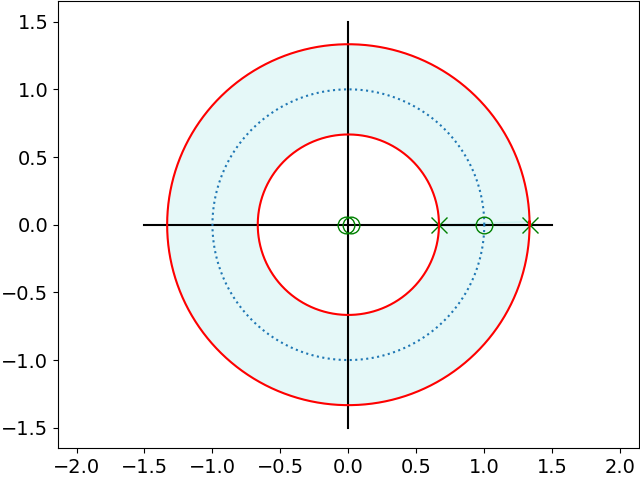
\includegraphics[width=80mm]{pz.png}
\end{center}
}

\end{document}